\documentclass[a4paper, 10pt]{article}

\usepackage{cite}
\usepackage{color}
	\definecolor{gray}{rgb}{0.5,0.5,0.5}
\usepackage{datetime}
\usepackage{fancyvrb}
\usepackage{graphicx}
\graphicspath{{images/}}
\DeclareGraphicsExtensions{.pdf,.png}
%\usepackage{hyperref}
\usepackage{latexsym}
\usepackage{listings}
	\lstset{
		frame=single,
		numbers=left,
		numberstyle=\small\color{gray},
		tabsize=4,
		morekeywords={and, boolean, do, else, false, for, if, integer, mod, true, until, wait, while},
	}
\usepackage{multirow}
\usepackage{setspace}
\usepackage{url}

\def \todo{\textbf{\textcolor{yellow}{TODO}}}
\def \citationneeded{\textbf{\textcolor{yellow}{CITATION NEEDED}}}

\title{Development and Analysis of Barrier Protocols}
\author{Ronny Brendel\\Tutors: Sascha Kl\"uppelholz \& Marcus V\"olp}

\begin{document}
%%%%%%%%%%%%%%%%%%%%%%%%%%%%%%%%%%%%%%%%%%%%%%%%%%%%%%%%%%%%%%%%%%%%%%%%%%%%%%%
\pagenumbering{gobble}

\begin{titlepage}

\begin{center}
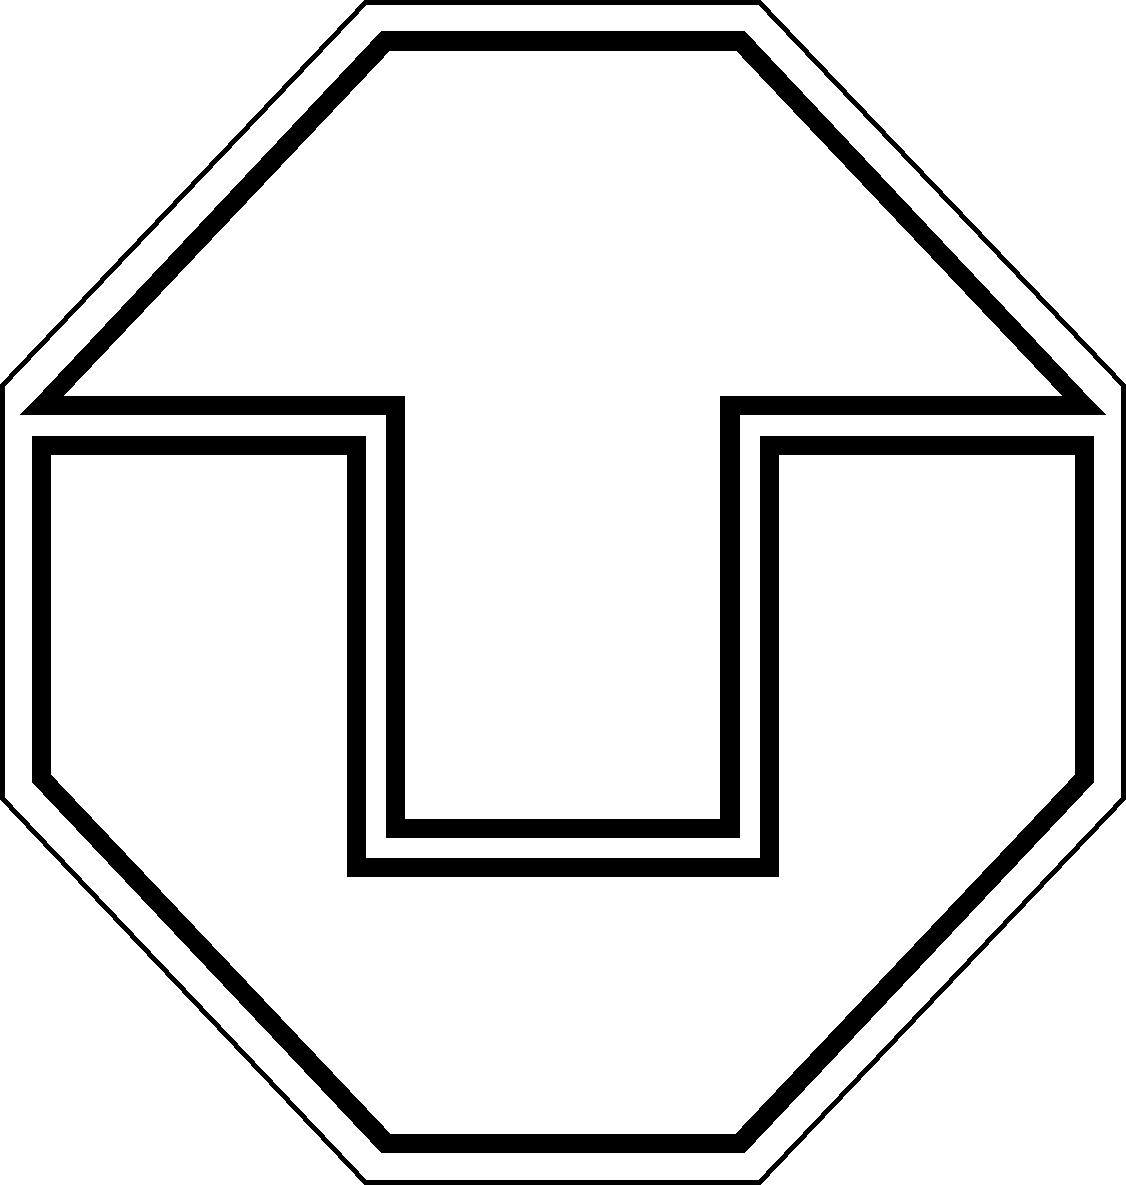
\includegraphics[width=3cm]{tu-logo}~\\[1cm]
\textsc{\LARGE Dresden University of Technology}\\[0.5cm]
\textsc{\Large Faculty of Computer Science}\\[0.2cm]
\textsc{\large Institute of Theoretical Computer Science}\\[0.2cm]
\textsc{\large Chair for Algebraic and Logical Foundations of Computer Science}\\[3cm]
\Huge Study's Thesis \\[1cm]
\huge Development and Analysis of Barrier Protocols\\[3cm]
\end{center}

\begin{flushleft} \large
	Author: Ronny Brendel \\
	Responsible university professor: Christel Baier \\
	Supervisors: Sascha Kl\"uppelholz \& Marcus V\"olp
\end{flushleft}

\vfill
\begin{flushright}
	\large October 2013
\end{flushright}

\end{titlepage}

\pagebreak
\newpage \thispagestyle{empty} \mbox{}
\pagebreak

%%%%%%%%%%%%%%%%%%%%%%%%%%%%%%%%%%%%%%%%%%%%%%%%%%%%%%%%%%%%%%%%%%%%%%%%%%%%%%%
\section*{Aufgabenstellung}

\pagebreak
\newpage \thispagestyle{empty} \mbox{}
\pagebreak

%%%%%%%%%%%%%%%%%%%%%%%%%%%%%%%%%%%%%%%%%%%%%%%%%%%%%%%%%%%%%%%%%%%%%%%%%%%%%%%
%\section*{Selbstst\"andigkeitserkl\"arung}
%Ich erkl\"are hiermit, dass ich die vorliegende Arbeit selbst\"andig und ohne Benutzung anderer als der angegebenen Hilfsmittel angefertigt habe. Die aus fremden Quellen w\"ortlich oder sinngem\"a\ss ~\"ubernommenen Gedanken sind als solche kenntlich gemacht. Ich erkl\"are ferner, dass ich die vorliegende Arbeit an keiner anderen Stelle als Pr\"ufungsarbeit eingereicht habe oder einreichen werde.

\section*{Statement of academic integrity}
I hereby declare that I prepared this thesis independently and without use of tools other than specified. Foreign thoughts, taken literally or in spirit, are marked as such. I also declare that I have not filed the present work at any other location or will submit it.

\pagebreak
\newpage \thispagestyle{empty} \mbox{}
\pagebreak

%%%%%%%%%%%%%%%%%%%%%%%%%%%%%%%%%%%%%%%%%%%%%%%%%%%%%%%%%%%%%%%%%%%%%%%%%%%%%%%
\renewcommand{\contentsname}{Table of contents}
\tableofcontents

\pagebreak
\newpage \thispagestyle{empty} \mbox{}
\pagebreak

%%%%%%%%%%%%%%%%%%%%%%%%%%%%%%%%%%%%%%%%%%%%%%%%%%%%%%%%%%%%%%%%%%%%%%%%%%%%%%%
\pagenumbering{arabic}
\section{Don't forget}
\begin{itemize}
	\item try all algorithms with processor counts $\neq 2^i$ especially dissemination
	\item explain use of 'thread' and 'process'
	\item explain constants used in listings somewhere
		\begin{itemize}
			\item threadCount/processCount
			\item threadIndex/processIndex
			\item ?more?
		\end{itemize}
\end{itemize}
%%%%%%%%%%%%%%%%%%%%%%%%%%%%%%%%%%%%%%%%%%%%%%%%%%%%%%%%%%%%%%%%%%%%%%%%%%%%%%%

\section{Introduction}
\begin{itemize}
	\item general introduction
	\item what is a barrier
	\item usage example for barriers. Reference rab00.
	\item motivation for researching barrier
	\item ?historical development?
	\item ?overarching thesis that will be worked on. Add a claim as recurrent theme.?
	\item what this report will be about
\end{itemize}


%%%%%%%%%%%%%%%%%%%%%%%%%%%%%%%%%%%%%%%%%%%%%%%%%%%%%%%%%%%%%%%%%%%%%%%%%%%%%%%
\section{Survey of means to implement barrier protocols}
\begin{itemize}
	\item evaluate what tools we have at our disposal to realize barrier protocols
	\item shared vs distributed memory
	\item the influence of latency
	\item bandwidth doesn't matter
\end{itemize}

%%%%%%%%%%%%%%%%%%%%%%%%%%%%%%%%%%%%%%%
\subsection{Shared memory}
\begin{itemize}
	\item atomic ops. most notably add-fetch, compare-swap \citationneeded
	\item normal load/store
	\item weaken memory model. most prominent release consistency \cite{gha90}
	\item hardware support e.g. SGI UV 2000 systems\cite{sgiuv2000}
\end{itemize}

%%%%%%%%%%%%%%%%%%%%%%%%%%%%%%%%%%%%%%%
\subsection{Distributed memory}
\begin{itemize}
	\item categories
		\begin{itemize}
			\item synchronous message passing
				\begin{itemize}
					\item relatively large overhead. Queueing. Waiting even when sending.
					\item not terribly interesting for developing new barriers
				\end{itemize}
			\item asynchronous message passing
				\begin{itemize}
					\item similar overhead as synchronous message passing. not necessarily waiting.
				\end{itemize}
			\item RDMA
				\begin{itemize}
					\item explain short what RDMA is and means. Coop between RAM and network card
					\item needs hardware support.
					\item less software overhead, since it is one sided. Less buffering.
					\item (a) coherent - remotely updated memory will be visible eventually
					\item (b) non-coherent - no guarantee about visibility of remotely updated memory - needs active asking for changes by the remote end.
					\item ?RDMA most interesting for new protocols because it is one sided- no active interaction with the remote end.?
				\end{itemize}
			\item hardware support here is more usual business e.g. Earth Simulator\cite{earthsimulator}, IBM Blue Gene/L\cite{bluegenel}, IBM Blue Gene/Q\cite{bluegeneq}, low-cost custom\cite{hoefler2006b}
			\item lossy communication e.g. UDP. ?any examples for synchronization on lossy channels? \citationneeded
		\end{itemize}
	\label{why-only-mpi}
	\item we specifically look at MPI. Explain short why only MPI. MPI prevalent \citationneeded~in dist memory programming? low level api. Many other higher level APIs use it as a basis \citationneeded.
	\item MPI has synchronous message passing
		\begin{itemize}
			\item MPI\_Send (Ssend assumed), MPI\_Rsend (returns if no receiver is present), MPI\_Recv
			\item chapter 3.2 in \cite{mpi3}
		\end{itemize}
	\item MPI has asynchronous message passing
		\begin{itemize}
			\item MPI\_Isend
			\item MPI\_Irecv
			\item MPI\_Wait, MPI\_Test
			\item MPI\_Cancel
			\item chapter 3.7 in \cite{mpi3}
			\item writing into a buffer given to MPI\_Isend is undefined behaviour, whereas bsend buffers the input itself and the original buffer is free to be used again.
			\item sync and async message passing can be mixed e.g. MPI\_Isend with a matching MPI\_Recv
		\end{itemize}
	\item MPI has asynchronous collectives
		\begin{itemize}
			\item chapter 5.12 in \cite{mpi3}
			\item non-blocking collectives are not interesting, because everyone has to take part and no cancellation of anything is possible.
		\end{itemize}
	\item MPI has RDMA
		\begin{itemize}
			\item \todo probably way too complicated try to break it down. and bring in a continuous thread: possibilties for implementing barriers. maybe even make a short wrap up at the end of the section.
			\item chapter 11 in \cite{mpi3}
			\item major changes from MPI 2.2 to 3.0\cite{mpi3onesided}
			\item MPI 2.2 is bad for our purpose because
				\begin{itemize}
					\item MPI\_Put/MPI\_get data may be not visible in main memory until a window is synchronized with fence/complete/wait
					\item MPI\_Fence implies a barrier on the participating processes.
					\item MPI\_Complete/MPI\_Wait is a sync between fewer processes, but ultimately the same as fence
					\item MPI 3.0 is 1 year old. It is not yet realized by openmpi, but it is for mpich 3.0 and derivatives such as MVAPICH2, Cray MPT\cite{craympt}
					\item following we will only consider MPI 3.0
				\end{itemize}
			\item MPI 3.0
				\begin{itemize}
					\item only scratch surface of MPI 3.0 one sided communication, because:
						\begin{itemize}
							\item a lot of details, because of generality, optimizability
							\item complicated semantics
							\item many of the details make no striking difference in protocol design/analysis
						\end{itemize}
					\item MPI\_Win\_Allocate allocates remotely shared memory amoung the participating process. A process group is associated with a window.
					\item customizable attributes of windows (don't distingish between MPI\_Info and attributes for the sake of ease):
						\begin{itemize}
							\item no\_locks: no window locking will be used
							\item accumulate\_ops:
							\item ~~~-~same\_op: impl may assume that all concurrent accesses to the same target address are the same op
							\item ~~~-~same\_op\_no\_op: assume all concurrent accumulates calls to the same address are MPI\_NO\_OP -$\>$ allows lower protection for the implementation
							\item  upon window creation set MPI\_Info key accumulate\_ordering to zero or more of the following: rar, war, raw, waw -$\>$ optimization. raw (read after write is serialized) means a write from one process has to finish before a read issued by the same process can take place. Default is all of them (sequential consistency) which means that reads and writes issued by a process to a remote location are committed in program order. Applies only to accumulate, not put and get. Put and get within an epoch are unordered.
							\item MPI\_WIN\_MODEL: One cannot set the MPI\_WIN\_MODEL to MPI\_WIN\_SEPARATE and MPI\_WIN\_UNIFIED myself. You can only ask for it. It has been proposed for MPI 3.1 to include being able to set a minimum necessary level.
						\end{itemize}
					\item mpich 3.0.4 does MPI\_WIN\_UNIFIED.
					\item explain epochs somewhere (before window sync perhaps)
						\begin{itemize}
							\item an epoch is a period between two sync calls e.g. fences
							\item rma calls like put/get/acc can only be used in an access epoch
							\item "in active target communication a target window can be accessed by RMA operations
								only within an exposure epoch"
							\item each access epoch is matched with exactly one exposure epoch
							\item used to accumulate multiple calls etc -$\>$ efficiency
							\item ?perhaps omit the details of two distinct types of epochs, if possible?
						\end{itemize}
					\item window sync
						\begin{itemize}
							\item active vs passive target communication (\cite{mpi3} page 437)
							\item MPI\_Win\_Fence. Is a collective over all window group members. All outstanding RMA requests between group members will be finished. More specifically: All locally initiated RMA request will finish locally before the fence call returns. At the target those same RMA requests will be completed when their respective MPI\_Win\_Fence call returns.
								and started before the fence call will complete at that process before the fence call returns.
								They will be completed at their target before the fence call returns at the target.
							\item MPI\_Win\_Start, MPI\_Win\_Complete, MPI\_Win\_Post, and MPI\_Win\_Wait: similar to fence, but allows to specify the sync partners exactly, and distinguishes between "command-issuing" and "remotely-accessed" processes. start/complete starts and ends access periods, post and wait start and end exposure epochs.
							\item MPI\_WIN\_LOCK, MPI\_WIN\_UNLOCK: starts and ends access epochs. no exposure epoch. no explicit participation of remote end in synchronization
						\end{itemize}
					\item window sync assertions: NoPrecede, NoSucceed, NoStore, NoPut -$\>$ optimization
					\item MPI\_Put, MPI\_Get
					\item MPI\_Accumulate, MPI\_FetchAndOp (getaccumulate subsumed by f\&o), MPI\_CompareAndSwap
				\end{itemize}
		\end{itemize}
\end{itemize}

%%%%%%%%%%%%%%%%%%%%%%%%%%%%%%%%%%%%%%%%%%%%%%%%%%%%%%%%%%%%%%%%%%%%%%%%%%%%%%%
\section{Survey of currently used barriers}

%%%%%%%%%%%%%%%%%%%%%%%%%%%%%%%%%%%%%%%
\subsection{Shared memory systems}
\begin{itemize}
	\item explain short why only research in glibc and gnu openmp. closed source intel, microsoft, portland pgi, pathscale. pthreads und openmp open source und weit verbreitet. ?llvm?
	\item gnu openmp
		\begin{itemize}
			\item gcc 4.8.0, linux
			% gnu-openmp/gcc-4.8.0/libgomp/libgomp.h
			% gnu-openmp/gcc-4.8.0/libgomp/barrier.c
			% gnu-openmp/gcc-4.8.0/libgomp/config/linux/
			% gnu-openmp/gcc-4.8.0/libgomp/config/linux/bar.h
			% gnu-openmp/gcc-4.8.0/libgomp/config/linux/bar.c
			% gnu-openmp/gcc-4.8.0/libgomp/config/linux/futex.h (cpu_relax)
			% gnu-openmp/gcc-4.8.0/libgomp/config/linux/wait.h
			\item central counter barrier with atomic add and fetch
			\item listing~\ref{listing:central-counter-no-reset}
				\begin{figure}[htbp]
					\centering
					\begin{minipage}
\centering
\begin{lstlisting}[mathescape, linewidth=10.4cm]
shared variables: integer barrier := threadCount
$\listingrule{10.4cm}$

atomic{barrier := barrier - 1}

wait until barrier = 0
\end{lstlisting}
\end{minipage}

					\caption{Pseudo code of the central counter barrier}
					\label{listing:central-counter-no-reset}
				\end{figure}

			\item backoff via a spin-counter $\sim$ 3ms. architecture specific. lowers spincount if cpucount $<$ threadcount. futexes. kernel based mutexes. wait queues. sleeping.
			\item reset built in. last one to enter resets the barrier.
		\end{itemize}
	\item glibc's new pthreads library
		\begin{itemize}
			\item version 2.17. is in my ubuntu raring 13.04.
			% glibc/nptl/sysdeps/pthread/pthread.h
			% glibc/nptl/pthread_barrier_*
			% glibc/nptl/sysdeps/unix/sysv/linux/internaltypes.h
			\item central counter with explicit locking instead of atomic add-fetch
			\item back-off through futexes (without spinning before)
			\item reset handled automatically (upon leaving the barrier every thread increments (atomically) the barrier by 1 so that it is max in the end)
		\end{itemize}
\end{itemize}

%%%%%%%%%%%%%%%%%%%%%%%%%%%%%%%%%%%%%%%
\subsection{Distributed memory systems}
\begin{itemize}
	\item why only MPI. Already explained in section~\ref{why-only-mpi}.
	\item openmpi
		\begin{itemize}
			\item version 1.7. not yet released.
			% ompi/mca/coll/tuned/coll_tuned_barrier.c :
			% ompi_coll_tuned_barrier_intra_recursivedoubling,
			% ompi_coll_tuned_barrier_intra_bruck
			% ompi/mca/coll/tuned/coll_tuned_decision_fixed.c
			\item $n \neq 2^k \rightarrow$ dissemination\cite{hensgen1988} using sync sendrecv
			\item $n = 2^k \rightarrow$ recursive doubling (explanation e.g. in \cite{hoefler2005})
			\item back-off hard to determine. probably through OPAL\_THREAD\_(UN)LOCK in the end
			\item resetting (in both algorithms) not necessary since sendrecv sets up itself newly everytime.
			\item architecture specific for infiband. e.g. dissemination using rdma \cite{hoefler2006a}
			\item ~
				\begin{figure}[htbp]
					\centering
					\begin{lstlisting}[mathescape]
shared variables: boolean
                  barrier[processCount][processCount]
local variables:  integer dist
initialization:   barrier[*][*] := false

for dist := 1; dist < numThreads; dist := dist $\times$ 2 {
	to   := (processIndex + dist) (mod processCount)
	from := (processIndex - dist) (mod processCount)
	
	barrier[to][processIndex] := true
	
	wait until barrier[processIndex][from] = true
}
\end{lstlisting}


					\caption{Pseudo code of the dissemination barrier}
					\label{listing:dissemination-no-reset}
				\end{figure}
				things to explain
				\begin{itemize}
					\item each array (first index) is located on the respective process's memory
				\end{itemize}

		\end{itemize}
	\item mpich
		\begin{itemize}
			\item many mpi implementations are based on mpich (e.g. mvapich2, intel mpi, cray mpi,
			\item many can not be inspected because source is closed
			\item version 3.0.4. current today
			% src/mpi/coll/barrier.c : MPIR_Barrier_intra
			\item log2 Dissemination with sendrecv. same as openmpi
		\end{itemize}
	\item dissemination can also be used for shared memory\cite{hoefler2013}
\end{itemize}

%%%%%%%%%%%%%%%%%%%%%%%%%%%%%%%%%%%%%%%%%%%%%%%%%%%%%%%%%%%%%%%%%%%%%%%%%%%%%%%
\section{Three new barriers}
%%%%%%%%%%%%%%%%%%%%%%%%%%%%%%%%%%%%%%%
\subsection{NMG/Ronny}
\begin{itemize}
	\item ~
		\begin{figure}[htbp]
			\centering
			\begin{minipage}
\centering
\begin{lstlisting}[mathescape, linewidth=12.1cm]
constants:        meBit:=$2^{threadIndex}$, full:=$\sum_{i=0}^{threadCount-1}2^i$
shared variables: integer entry := 0, integer exit := 0,
                  boolean left := false
local variables:  integer copy
$\listingrule{12.1cm}$

if left = false {

	do {
		copy := (copy & $\sim$meBit) | entry
		if copy & meBit = 0 {
			copy  := copy | meBit
			entry := copy
		}
	} while copy $\neq$ full and left = false

	left := true
	exit := 0

} else if left = true {

	do {
		copy := (copy & $\sim$meBit) | exit
		if copy & meBit = 0 {
			copy := copy | meBit
			exit := copy
		}
	} while copy $\neq$ full and left = true

	left  := false
	entry := 0
}
\end{lstlisting}
\end{minipage}

			\caption{Pseudo code of nmg+ronny's barrier}
			\label{listing:nmg-ronny-with-reset}
		\end{figure}

		things to explain
		\begin{itemize}
			\item ~
		\end{itemize}

	\item reference old work
	\item mention errors -$>$ correction
	\item improvement (remember others)
	\item still slow and inefficient
	\item resetting included in the protocol
	\item advantage: no atomic ops
	\item + variations: array based for more than 64 threads
\end{itemize}

%%%%%%%%%%%%%%%%%%%%%%%%%%%%%%%%%%%%%%%
\subsection{Ronny's simple barrier for shared memory}
\begin{itemize}
	\item ~
		\begin{figure}[htbp]
			\centering
			\documentclass[class=article, border=10pt]{standalone}

\usepackage[latin1]{inputenc}
\usepackage{tikz}
\usetikzlibrary{shapes,arrows,positioning}
\begin{document}
\pagestyle{empty}

%styles
\tikzstyle{->}   = [draw, -latex']
\tikzstyle{o}    = [draw, circle]
\tikzstyle{box}  = [draw, rectangle, rounded corners]

\begin{tikzpicture}[node distance = 2.0cm, auto]


% preamble
\node [box, align=left] (pre)  {
	\begin{minipage}{12cm}
		\begin{itemize}
			\item constants:
				\begin{itemize}
					\item[] \textbf{integer} nthreads {\color{gray} number of threads}
					\item[] \textbf{integer} me \color{gray} thread identificator (0..nthreads-1)
				\end{itemize}
			\item shared variables:
				\begin{itemize}
					\item[] \textbf{boolean} barrier[0..nthreads-1] \color{gray}each element on an own cacheline
				\end{itemize}
			\item local variables:
				\begin{itemize}
					\item[] \textbf{integer} i
				\end{itemize}
			\item initialize:
				\begin{itemize}
					\item[] barrier[*] := false
					\item[] i := 0
				\end{itemize}
		\end{itemize}
	\end{minipage}
};

% nodes
\node [o, below of=pre, draw=none, yshift=-2cm]  (init) {};
\node [o, below of=init]                         (1)    {};
\node [o, below of=1]                            (2)    {};
\node [o, below of=2]                            (3)    {};
\node [o, below of=3, draw=none]                 (done) {};

%  edges
\path [->] (init) edge                                      node       {\color{gray}(work period)}                                (1);
\path [->] (1)    edge                                      node       {barrier[me] := true \color{gray}(local shared write)}     (2);
\path [->] (2)    edge [loop, distance=2cm, out=45, in=-45] node       {barrier[i] $\ne$ true : i := 0 \color{gray}(remote shared read)} (2);
\path [->] (2)    edge                                      node       {else : i := i + 1 \color{gray}(remote shared read)}       (3);
\path [->] (3)    edge [out=180, in=180]                    node[left] {i $<$ nthreads}                                           (2);
\path [->] (3)    edge                                      node       {else}                                                     (done);

\end{tikzpicture}

\end{document}



			\caption{Pseudo code of ronny's simple barrier}
			\label{listing:ronny-simple-no-reset}
		\end{figure}

		things to explain
		\begin{itemize}
			\item ~
		\end{itemize}

	\item advantage: no atomic ops
	\item much shared read communication but low computation overhead
	\item ?discuss a variant with reset?, if not at least mention that reset is not handled here
	\item + variations: remember first few, remember last few, more?
\end{itemize}

%%%%%%%%%%%%%%%%%%%%%%%%%%%%%%%%%%%%%%%
\subsection{Ronny's fancy barrier for dist memory}
\begin{itemize}
	\item ~
		\begin{figure}[htbp]
			\centering
			\begin{minipage}
\centering
\begin{lstlisting}[mathescape, linewidth=11.5cm]
constants:        me := processIndex, meBit := $2^{me}$,
                  full := $\sum_{i=0}^{\mathit{processCount}-1}2^i$
shared variables: integer barrier[processCount]
initialization:   barrier[*] := full
$\listingrule{11.5cm}$

barrier[me] := full & $\sim$meBit;

i := processIndex + 1 (mod processCount)
do {
	while barrier[me] & $2^i$ = 0 and i < processCount {
		i := i + 1
	}

	if i < processCount {
		barrier[me] := barrier[me] & barrier[i]
	} else {
		i := 0
	}
} while barrier[me] $\neq$ 0
\end{lstlisting}
\end{minipage}

			\caption{Pseudo code of ronny's fancy barrier}
			\label{listing:ronny-fancy-no-reset}
		\end{figure}

		things to explain
		\begin{itemize}
			\item each array element is located in its own process - dist mem
		\end{itemize}

	\item advantage: no atomic ops
	\item trades computational overhead for, less shared read communication than the simple variant
	\item ?discuss a variant with reset?, if not at least mention that reset is not handled here
	\item + variations: which?
\end{itemize}

%%%%%%%%%%%%%%%%%%%%%%%%%%%%%%%%%%%%%%%%%%%%%%%%%%%%%%%%%%%%%%%%%%%%%%%%%%%%%%%
\section{Analysis and comparison of the contenders}

\begin{itemize}
	\item pick central counter barrier as contender for shared mem
	\item pick dissemination as contender for distributed mem
\end{itemize}

%%%%%%%%%%%%%%%%%%%%%%%%%%%%%%%%%%%%%%%
\subsection{Prose}
\begin{itemize}
	\item meantion that no backoff is used
\end{itemize}

\subsubsection{central counter for shared memory}
\subsubsection{ronny simple for shared memory}
\subsubsection{dissemination for distributed memory}
\begin{itemize}
	\item number of messages sent vs the minimum necessary
	\item progress problem when one process is missing
	\item meantion the xeon phi work of TH
\end{itemize}
\subsubsection{ronny fancy for distributed memory}
\begin{itemize}
	\item ?number of messages sent?
\end{itemize}

%%%%%%%%%%%%%%%%%%%%%%%%%%%%%%%%%%%%%%%
\subsection{Benchmarks}
\begin{itemize}
	\item central counter vs ronny simple
	\item do not do dissemination vs ronny fancy
	\item ?rapl?
\end{itemize}

%%%%%%%%%%%%%%%%%%%%%%%%%%%%%%%%%%%%%%%
\subsection{Model checking}
\subsubsection{Qualitative Properties (correctness)}
\begin{itemize}
	\item threads may only exit the barrier if all threads are present
	\item the protocol must always terminate, or in other words: if all threads are present, they will all exit the barrier in a finite amount of time"
\end{itemize}
\subsubsection{Quantitative Properties}
\begin{itemize}
	\item central counter vs ronny simple
	\item dissemination vs ronny fancy
\end{itemize}

%%%%%%%%%%%%%%%%%%%%%%%%%%%%%%%%%%%%%%%%%%%%%%%%%%%%%%%%%%%%%%%%%%%%%%%%%%%%%%%
\section{Proposal: Dissecting barrier protocols into orthogonal parts}
Cut up existing barriers into orthogonal pieces. Analyse and replace them independently.
\begin{itemize}
	\item more or less intelligence / bandwidth/latency vs additional calculations
	\item 
		reset

		\begin{itemize}
			\item how is resetting handled in currently used barriers?
			\item switching between barriers using a variable (as in the mcquire/ronny barrier - 'left' variable)
			\item use 3 barriers reset barrier x+2 when you finished barrier x. switch between the barriers by checking if barrier x+2 is reset or not (as in central-counter-with-reset)
			\item if variable space permits it you can also change the variables to 'counters' and modify all checks to ask for numbers modulo round + a check that you are in the proper round
		\end{itemize}

	\item back-off
\end{itemize}

%%%%%%%%%%%%%%%%%%%%%%%%%%%%%%%%%%%%%%%%%%%%%%%%%%%%%%%%%%%%%%%%%%%%%%%%%%%%%%%
\section{Conclusion}
\begin{itemize}
	\item condense results into a small passage
	\item ?repeat claim - overarching thesis - present an answer?
\end{itemize}

%%%%%%%%%%%%%%%%%%%%%%%%%%%%%%%%%%%%%%%%%%%%%%%%%%%%%%%%%%%%%%%%%%%%%%%%%%%%%%%
\section{Future Work}
\begin{itemize}
	\item evaluate back-off strategies. mwait.
	\item model check more and bigger. symmetrie reduction. partial order reduction.
	\item explore variations of ronny's barriers
		\begin{itemize}
			\item use remote write \& local read instead of local write \& remote read, because remote writing is preferred on some platforms, e.g. on the Epiphany\cite{epiphany}.
		\end{itemize}
\end{itemize}


%%%%%%%%%%%%%%%%%%%%%%%%%%%%%%%%%%%%%%%%%%%%%%%%%%%%%%%%%%%%%%%%%%%%%%%%%%%%%%%
\appendix

%%%%%%%%%%%%%%%%%%%%%%%%%%%%%%%%%%%%%%%%%%%%%%%%%%%%%%%%%%%%%%%%%%%%%%%%%%%%%%%
\pagebreak
\section{Appendix}
\subsection{e.g. source code, model source}

%%%%%%%%%%%%%%%%%%%%%%%%%%%%%%%%%%%%%%%%%%%%%%%%%%%%%%%%%%%%%%%%%%%%%%%%%%%%%%%
\pagebreak
\section{Glossary}

%%%%%%%%%%%%%%%%%%%%%%%%%%%%%%%%%%%%%%%%%%%%%%%%%%%%%%%%%%%%%%%%%%%%%%%%%%%%%%%
\pagebreak
\section{Bibliography}
\renewcommand\refname{\vskip -1cm} %TODO fine tune perhaps
\nocite{*} % insert not cited references
\bibliographystyle{abbrv}
\bibliography{bibliography}{}

%%%%%%%%%%%%%%%%%%%%%%%%%%%%%%%%%%%%%%%%%%%%%%%%%%%%%%%%%%%%%%%%%%%%%%%%%%%%%%%
\pagebreak
\section{List of Figures}
\renewcommand{\listfigurename}{\vskip -1cm} %TODO fine tune perhaps
\listoffigures

%%%%%%%%%%%%%%%%%%%%%%%%%%%%%%%%%%%%%%%%%%%%%%%%%%%%%%%%%%%%%%%%%%%%%%%%%%%%%%%
\pagebreak
\section{List of Tables}
\renewcommand{\listtablename}{\vskip -1cm} %TODO fine tune perhaps
\listoftables

\end{document}
